\section{Architecture and Building Blocks}
\label{sec:gns3architecture}

A good written, comprehensive description of the GNS3 architecture and technical details is lacking.
There is a page, on the online developers-oriented documentation~\cite{gns3devarch}, which presents a very simple diagaram, reproduced\footnote{Dashed strokes are added by the author of the dissertation to provide extra information} on figure~\ref{fig:gns3-docs-arch}.
Even the two published books that exist on the project~\cite{gns3netsimguide,thebookofgns3} are omissive or very brief, not allowing for gaining an in-depth knowledge, necessary to understand the possible issues of performance, resource consumption, scalability, and functional limitations that GNS3 may suffer from.
Going from the simple diagram that was mentioned, towards a more complete reference is one of this dissertation's efforts.

To accomplish such effort, a precious resource has been the ``paraofficial'' videos available via YouTube, mostly by David Bombal, an instructor and close collaborator of the GNS3 organization, namely a comprehensive overview of the architecture (compared with the functionality) of GNS3 by its creator, Jeremy Grossmann~\cite{ytgns3arch22}, and essentially are not anywhere else, at least from authoritative sources. % TODO do nothing with \footnote{\url{https://www.youtube.com/channel/UCP7WmQ_U4GB3K51Od9QvM0w}} ?

% Figure fig:gns3-docs-arch
\begin{figure}
  \centering
  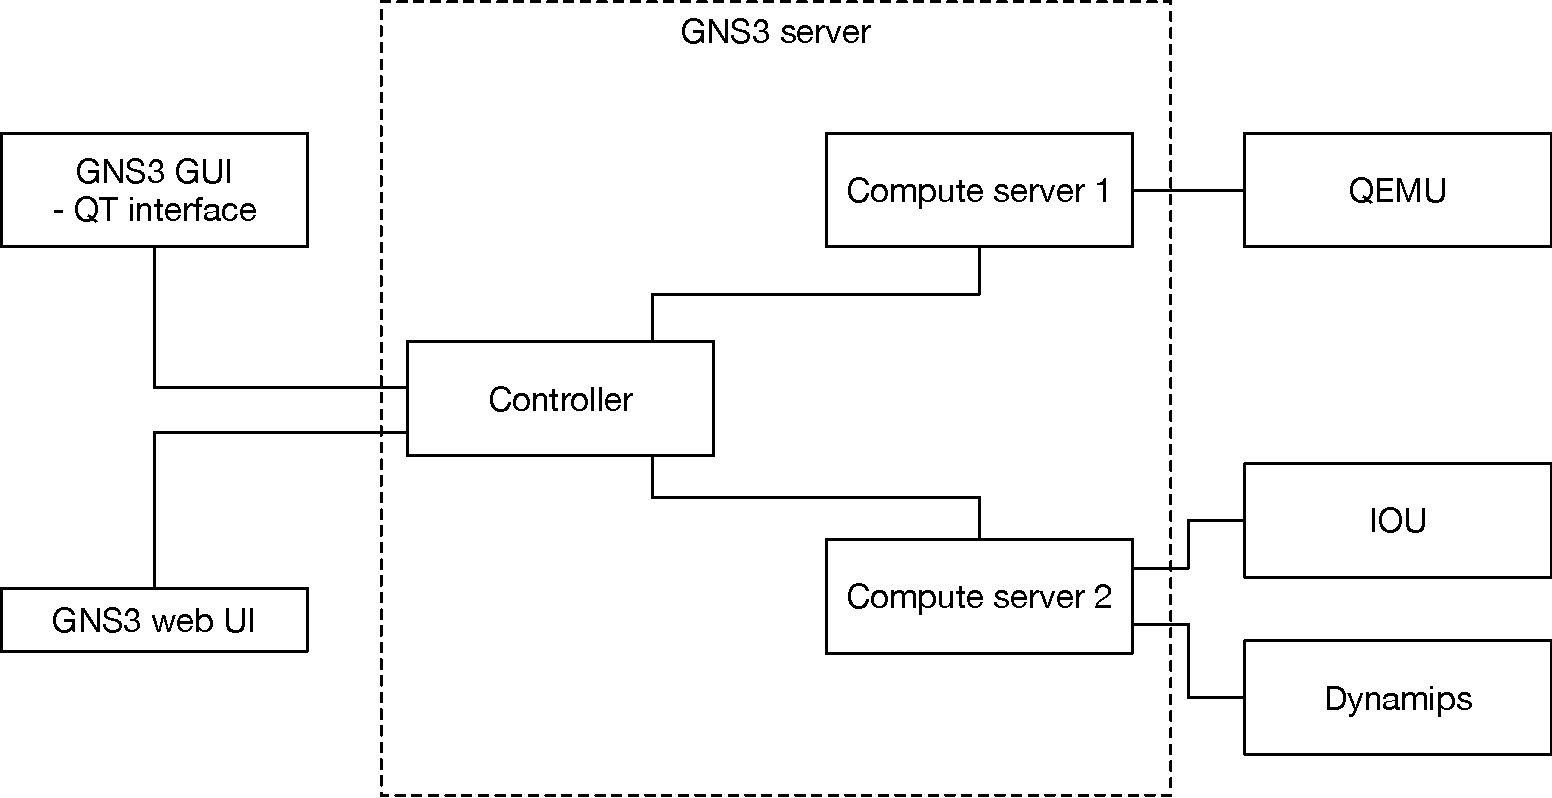
\includegraphics[width=0.8\textwidth]{gns3-docs-arch}
  \caption{The architecture of GNS3 (adapted from the official documentation)}
  \label{fig:gns3-docs-arch}
\end{figure}


\subsection{The Simple Client-Server Perspective}
\label{subsec:gns3clientserver}

GNS3 works, first and foremost, as a client-server application.
The standard installation for desktop provides all the necessary components to fully(-ish) work on that physical machine, but the client doesn't have to be, and in many real scenarios isn't, running on the same host as the server.
However, in fact, a \textbf{topology}---the name GNS3 gives to its ``projects,'' which comprises of nodes (emulated/virtualized routers, switches, \gls{sdn}-controllers, virtual PCs, interfaces for hardware network connections)---can be running in different machines, even on the ``backend'' side itself, as will be seen.

The \textbf{GNS3 server} exposes a public \gls{rest} \gls{api}, documented in~\cite{gns3devarch}, which is the way any client edits the opened topology or performs actions on the nodes contained therein, or in the GNS3 running environment.
GNS3 server, described more thoroughly afterwards, is the brains and central point of topology opened and in-execution.
It has first-hand knowledge of events that occur in the nodes, their status, their interfaces' status, and communicates with the several means existing to actually provide the \emph{emulation} for each specific node.
All of this will be analyzed and explained posteriorly.
For now, it suffices to see it as a central point, accessible by any number of clients, of a running topology.

To interact with the system---i.e. editing a topology or performing actions on nodes which are all the items in the topology, that can be connected via links---, one or more users simultaneously can utilize a graphical client, usually GNS3 GUI. The \textbf{GNS3 GUI}, part of a standard installation on any desktop operating system, namely macOS, a desktop Linux distribution (official repositories for Ubuntu exist), or Windows,\footnote{\url{https://gns3.com/software/download}} is a cross-platform application developed using the Qt graphical toolkit~\cite{qttoolkit}.
Users may also use a web UI (somewhat limited yet), or any tool, user-driven or automatic, programmed to send requests and receive responses according to the aforementioned \gls{rest} specification.
The official clients, bundled with the GNS3 installation packages for desktop environments, GNS3 GUI and the official web UI, show an in-real-time view of the topology---e.g. the status of virtual network interfaces, or changes made by other client---thanks to WebSockets server-to-client up-calls~\cite{ytgns3arch22}. % TODO link WS to the glossary, when definition is available

% Figure fig:gns3-2hosts2routers-macOS
\begin{figure}
  \centering
  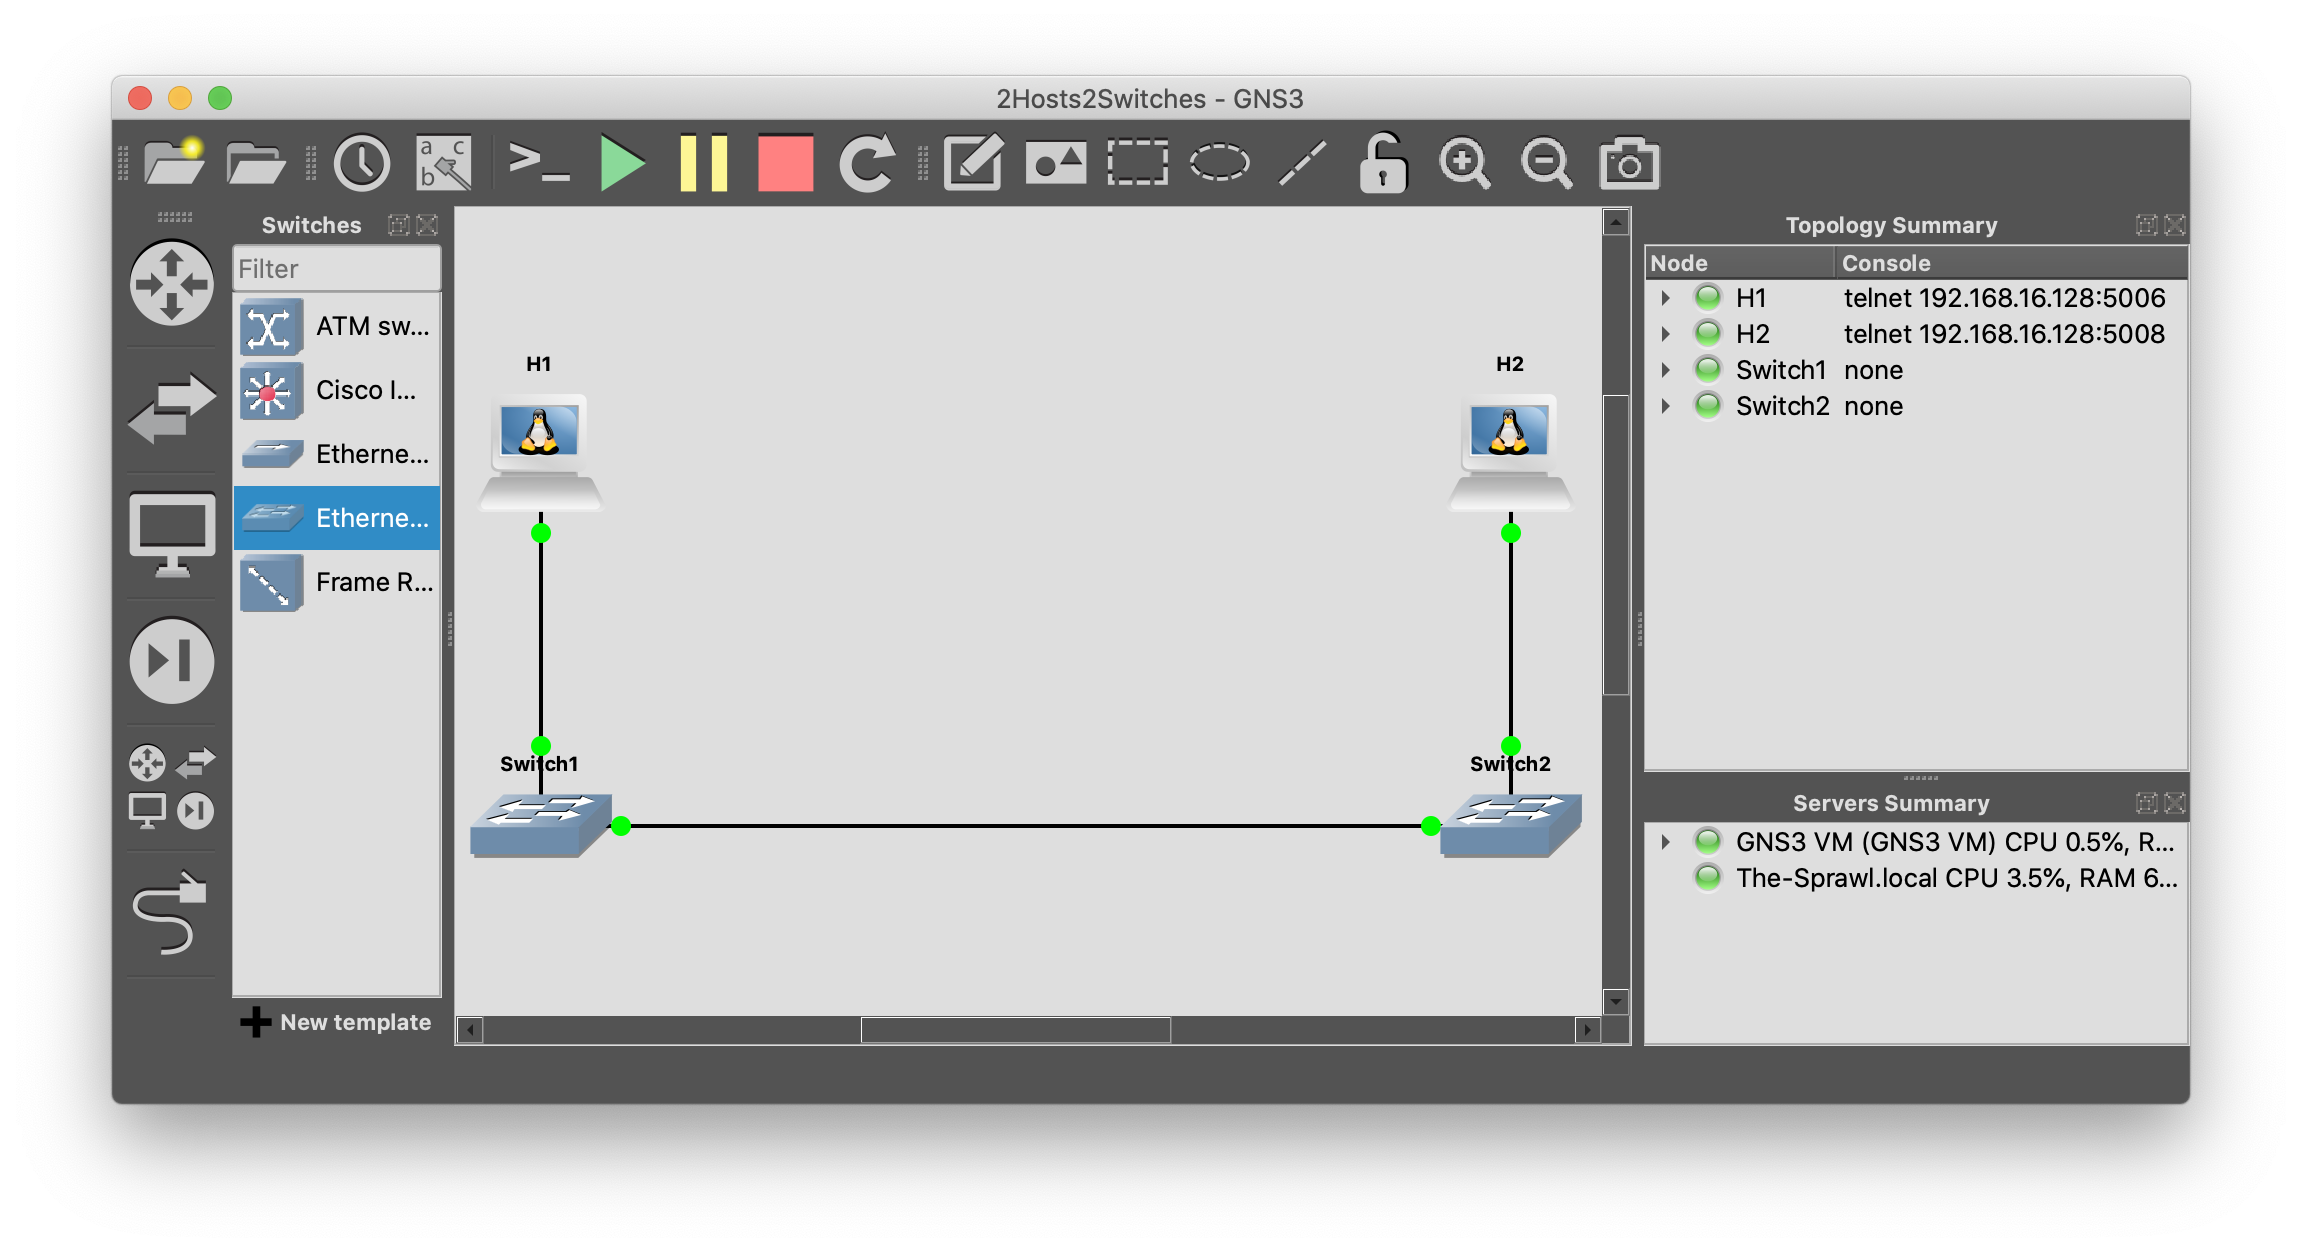
\includegraphics[width=0.8\textwidth]{gns3-2hosts2routers-macOS}
  \caption{Simple topology with only two switches and two virtual PCs as seen on the GUI in macOS}
  \label{fig:gns3-2hosts2routers-macOS}
\end{figure}


\subsection{The GNS3 Server---Distributed}
\label{subsec:gns3serverindetail}

The GNS3 server is a program with a code-base independent from other parts of the project.
The software package \texttt{gns3-server} can be obtained from official repositories for Linux systems to install it on servers without video interface, with users running some of the already mentioned clients in their laptops or desktop computers.
It is also possible to obtain a VMware ESXi image to directly spin-up a GNS3 server ready machine on an virtualized infrastructure.

The same program behaves as two different roles, both of which are necessary to get the GNS3 system working.

\begin{itemize}
	\item The \textbf{controller node}, or just ``controller,'' of which there can only be one instance per running topology, and is ``[its] decision point'' (Jeremy Grossmann's words); the process responsible for fulfilling the client's requests and postback real-time information to them and know the hosts where nodes may be running.
	\item The \textbf{compute node}, referred to simply as ``compute'' too, which, for one running topology, can be running $N$ times, one per each machine (physical or virtual) taking care of emulating one or more topology nodes (again: switches, routers, etc.).
	It is this separation and the ability to have multiple compute nodes that allows GNS3 to be configured in a way that can serve arbitrarily large topologies, since the cost in resources of an increasing number of ``live'' nodes can be balanced among an also increasing number of servers running a compute node.
\end{itemize}

When the server is running on a single host, one \texttt{gns3-server} program instance (i.e. process) performs both roles, controller and compute.
However, when the server is distributed across one or more machines, communication between the controller and the computes on other hosts happens through a \gls{rest} \gls{api}.
That \gls{api} is a private or internal one, unlike the one for client-server, and there isn't a programmer's manual for developing with it.
Only the (single) controller is supposed to communicate with each process acting as compute.

% end of section gns3architecture
